% !TeX root = exercises_main.tex
\section*{Task 1: Introductory Example}

Consider the following switched ODE

\begin{equation}\label{eq:task1_rhs}
\begin{aligned}
\frac{d}{dt}x_1(t) &= 
\begin{cases}
	q_1(t), & \text{if } x_1(t) \leq 750 \\
	q_1(t) - q_2(t),  & \text{if } x_1(t) > 750 \\
\end{cases} \\
\frac{d}{dt}x_2(t) &= 
\begin{cases}
	0, & \text{if } x_1(t) \leq 750 \\
	-300, & \text{if } 750 < x_1(t) < 800 \\
	0, & \text{if } x_1(t) \geq 800 \\
\end{cases}
\end{aligned}
\end{equation}
where
\begin{equation}\label{eq:task1_rhs_helpers}
\begin{aligned}
q_1(t) &= \frac{50}{27}t^2 - \frac{100}{3}t + \frac{400}{3} \\
q_2(t) &= (1000 - x_2)(p_1(t-19) + p_2)
\end{aligned}
\end{equation}

\begin{enumerate}[label=\alph*)]
	
	\item \label{item:task1a} \textbf{Subtask:}\\
	Use \lstinline|ode45| to solve this system on the time interval $I = [0, 30]$ with initial conditions $x_1(0) = 0$ and $x_2(0) = 1000$. Use $p = (\frac{3}{4}, \frac{1}{4})$ as the parameter vector. \\
	Plot the solution. Does the solution look correct? Explain why \lstinline|ode45| produces this result. \\ \\
	\textbf{Steps:}
	\begin{enumerate}[label=\arabic*.]
		\item Implement the RHS in the file \texttt{rhsTask1.m} as described by \cref{eq:task1_rhs} and \cref{eq:task1_rhs_helpers}. Compute the values of $q_1(t)$ and $q_2(t)$ directly in the RHS as local variables \lstinline|q1| and \lstinline|q2| (do not implement them as separate functions).
		\item Set the integration time span, initial conditions and parameters in the file \texttt{runTask1.m}.
		\item Use \lstinline|ode45| to compute a solution. Remember to pass the RHS as an anonymous function \\\lstinline|@(t, y) rhsTaks1(t, y, p)|, which takes a timepoint and state vector and returns the derivative vector. Don't forget to provide the integration time span and initial conditions.
		\item Create a vector of timepoints where you will plot the solution using\\ \lstinline|t = linspace(tspan(1), tspan(end), 1000)|.
		\item Evalute the solution at the timepoints using \lstinline|y = deval(solution, t)|.
		\item Plot the solution using \lstinline|plot(t, y')|, which will plot both solution components into one plot. Notice that the solution vector must be transposed here with \lstinline|y'| because the \lstinline|plot| function plots data column-wise.
	\end{enumerate}

	\item \textbf{Subtask:}\\
	Solve the system from subtask \ref{item:task1a} again, but this time with a maximum integrator step size of $0.1$. \\
	Plot the solution. Does the solution look correct? Explain why \lstinline|ode45| produces this result. \\ \\
	\textbf{Steps:}
	\begin{enumerate}[label=\arabic*.]
		\item Add the maximum step size to the integrator options using \\
		\lstinline|options = odeset(..., 'MaxStep', 0.1)|.
		\item Run your code from subtask \ref{item:task1a} with the new options.
	\end{enumerate}
	
	\item Now, solve this system using IFDIFF. What changed in comparison to a)? Use the same function header and implementation of the helper functions as mentioned in a)
	
	\item Let's see how the solution responds to changes in the initial values: Plot the sensitivities of the solution using \verb|plotSensitivities_odexx(sol, @rhsTask1, p, @ode45, options)|. Do they look correct?
	
	\item Plot the sensitivities of the solution with IFDIFF using \verb|plotSensitivities_ifdiff()|. How do the sensitivities differ from the sensitivities you previously computed in Task 1?
	
	\item Now, compute and plot the sensitivities of this solution. What do you notice?
	
\end{enumerate}

For reference, your solution and sensitivity plots with IFDIFF should look like the following:
\newpage
\begin{figure}[h!]
	\centering
	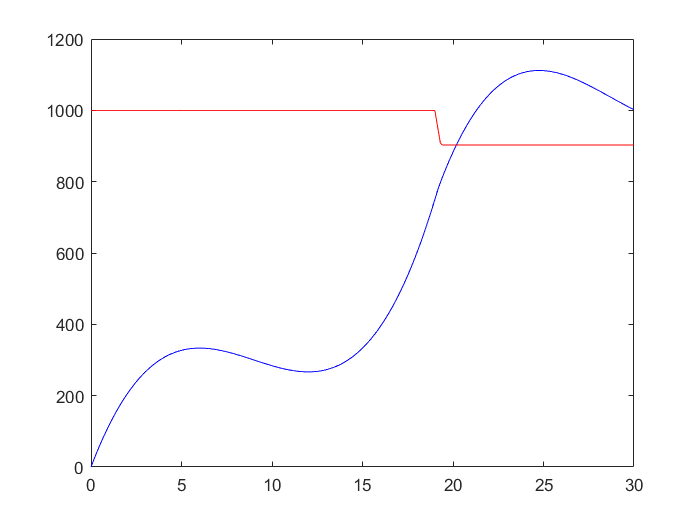
\includegraphics[width=0.75\linewidth]{Plots/task1solution_ifdiff.png}
	\caption{Solution plot for c)}
\end{figure}

\begin{figure}[h!]
	\centering
	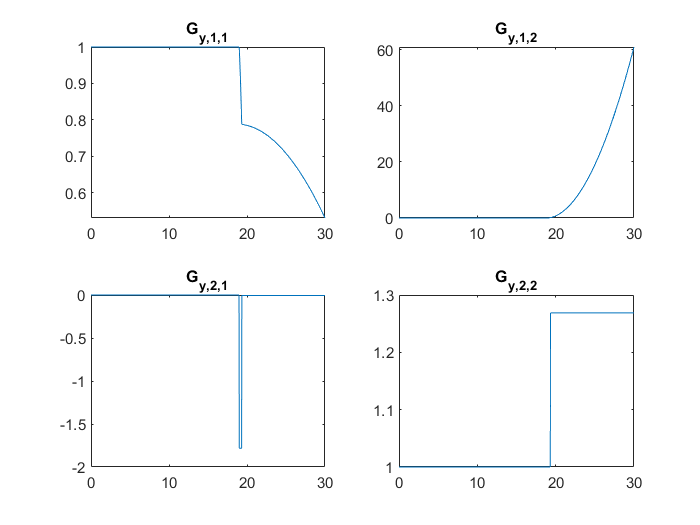
\includegraphics[width=0.75\linewidth]{Plots/task1sensitivities_ifdiff.png}
	\caption{Sensitvities for d)}
\end{figure}

\newpage

